\subsection{BERT}
\label{subsec:BERT_methods}
In this section, we describe the implementation of the same two Italian pre-trained BERT models used in \ref{subsec:Embeddings} to extract contextual embeddings, Italian BERT and AlBERTo. The aim is to verify if the implementation of these models as binary classifiers, opportunely fine-tuned for the task at hand, proves to yield better performances than the more traditional models implemented beforehand.

After loading the datasets, we loaded the pre-trained model's tokenizer using the Hugging Face Transformer library. We then prepared the text by adding the [CLS] token at the beginning of each sequence, to allow for correct processing by the tokenizer, which converts the sequences in tokens that match its training data. Since BERT exploits fixed-lenght encoding, we set the maximum sequence lenghts for our sentences (128 for the training set, 512 for the test sets). We also added the required [SEP] token at the end of each sequence. The BERT tokenizer was then used to convert each token into an integer index that points to the proper embedding in the BERT vocabulary. Sentences shorter than the fixed maximum lenght were padded with zeros. Each token also received an attention mask, with 1 if it is a real token and 0 if it is padding.

After reserving 10\% of the training set for validation, we created PyTorch Dataloaders for each set (train, validation, and the two test sets), to provide batches of 32 data sequences for the model to process in parallel.

We then proceeded to load the pre-trained model with a single linear classification layer added on top. We retrieved the model's training parameters and set the remaining hyperparameters for tuning as shown in Table \ref{tab:training_params}. We then proceeded to train and evaluate the model after each training epoch. For both models, we first tested 4 epochs and different learning rates for the Adam optimizer, but by plotting the loss trend on the training and evaluation dataset per epoch, we could see how in each experiment the training loss would decay, but the validation loss would increase after the second epoch (cf. an example in Figure \ref{fig:example_losses}) . This is a signal of overfitting: the model is not really learning from the training set, but rather memorizing it, which hurts its capability to generalize on the validation set.

Therefore, we decided to set the epochs to two, even if the training loss was still on a decreasing trend. 

\begin{table}[h]
    \centering
    \begin{tabular}{|l|c|}
    \hline
    \textbf{Parameter} & \textbf{Values} \\ \hline
    Epochs & 2\\ \hline
    Learning rate & 2e-5\\ \hline
    Weight Decay & 0.01 \\ \hline
    Batch-size & 32 \\ \hline
    \end{tabular}
    \caption{BERT's hyperparameters for tuning}
    \label{tab:training_params}
\end{table}

\begin{figure}
    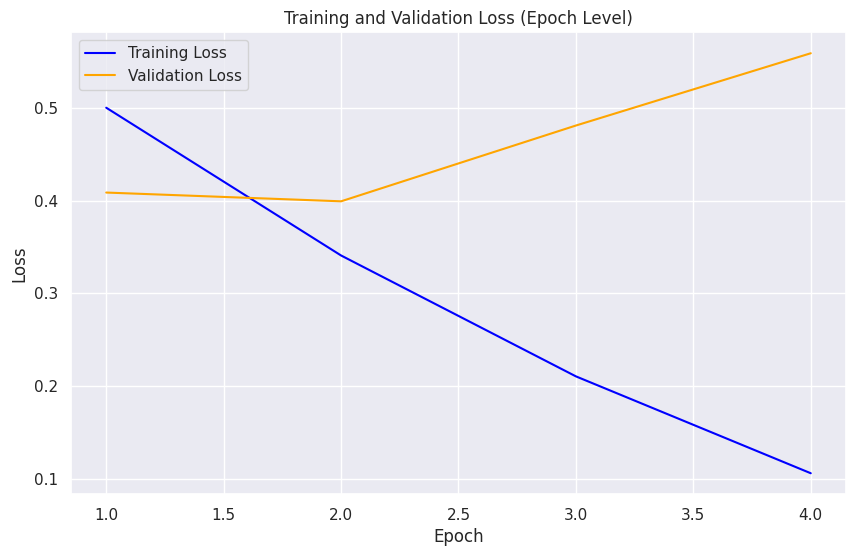
\includegraphics[width=\columnwidth]{../../results/images/alberto_losses_4epochs.png}
    \caption{AlBERTo Training and Validation Loss trend (LR = 2e-5, Epochs = 4).}
    \label{fig:example_losses}
\end{figure}